% ------------------------------------------------------------------------
% ------------------------------------------------------------------------
% Modelo UFSC para Trabalhos Academicos (tese de doutorado, dissertação de
% mestrado) utilizando a classe abntex2
%
% Autor: Alisson Lopes Furlani
% 	Modificações:
%	- 27/08/2019: Alisson L. Furlani, add pacote 'glossaries' para listas
%   - 06/11/2019: Luiz-Rafael Santos, modifica para Trabalho de Conclusão de Curso
% ------------------------------------------------------------------------
% ------------------------------------------------------------------------

\documentclass[
	% -- opções da classe memoir --
	12pt,				% tamanho da fonte
	%openright,			% capítulos começam em pág ímpar (insere página vazia caso preciso)
	oneside,			% para impressão no anverso. Oposto a twoside
	a4paper,			% tamanho do papel. 
	% -- opções da classe abntex2 --
	chapter=TITLE,		% títulos de capítulos convertidos em letras maiúsculas
	section=TITLE,		% títulos de seções convertidos em letras maiúsculas
	%subsection=TITLE,	% títulos de subseções convertidos em letras maiúsculas
	%subsubsection=TITLE,% títulos de subsubseções convertidos em letras maiúsculas
	% -- opções do pacote babel --
	english,			% idioma adicional para hifenização
	%french,				% idioma adicional para hifenização
	%spanish,			% idioma adicional para hifenização
	brazil				% o último idioma é o principal do documento
	]{abntex2}

\usepackage{setup/ufscthesisA4-alf}

% ---
% Filtering and Mapping Bibliographies
% ---
% Pacotes de citações
% ---
\usepackage{csquotes}
\usepackage[backend = biber, style = abnt]{biblatex}
% FIXME Se desejar estilo numérico de citações,  comente a linha acima e descomente a linha a seguir.
% \usepackage[backend = biber, style = numeric-comp]{biblatex}

\setlength\bibitemsep{\baselineskip}
\DeclareFieldFormat{url}{Disponível~em:\addspace\url{#1}}
\NewBibliographyString{sineloco}
\NewBibliographyString{sinenomine}
\DefineBibliographyStrings{brazil}{%
	sineloco     = {\mkbibemph{S\adddot l\adddot}},
	sinenomine   = {\mkbibemph{s\adddot n\adddot}},
	andothers    = {\mkbibemph{et\addabbrvspace al\adddot}},
	in			 = {\mkbibemph{In:}}
}

\addbibresource{aftertext/references.bib} % Seus arquivos de referências

% ---
\DeclareSourcemap{
	\maps[datatype=bibtex]{
		% remove fields that are always useless
		\map{
			\step[fieldset=abstract, null]
			\step[fieldset=pagetotal, null]
		}
		% remove URLs for types that are primarily printed
%		\map{
%			\pernottype{software}
%			\pernottype{online}
%			\pernottype{report}
%			\pernottype{techreport}
%			\pernottype{standard}
%			\pernottype{manual}
%			\pernottype{misc}
%			\step[fieldset=url, null]
%			\step[fieldset=urldate, null]
%		}
		\map{
			\pertype{inproceedings}
			% remove mostly redundant conference information
			\step[fieldset=venue, null]
			\step[fieldset=eventdate, null]
			\step[fieldset=eventtitle, null]
			% do not show ISBN for proceedings
			\step[fieldset=isbn, null]
			% Citavi bug
			\step[fieldset=volume, null]
		}
	}
}
% ---

% ---
% Informações de dados para CAPA e FOLHA DE ROSTO
% ---
% FIXME Substituir 'Nome completo do autor' pelo seu nome.
\autor{MATEUS MISCHEL LODI}
% FIXME Substituir 'Título do trabalho' pelo título da trabalho.
\titulo{RELATÓRIO FINAL IC VOLUNTÁRIO}
% FIXME Substituir 'Subtítulo (se houver)' pelo subtítulo da trabalho.  
% Caso não tenha substítulo, comente a linha a seguir.
\subtitulo{IMPLEMENTAÇÃO DE UM MODELO NUMÉRICO DO SISTEMA ELETROMECÂNICO DE UM COMPRESSOR LINEAR PARA REFRIGERAÇÃO DOMÉSTICA}
% FIXME Substituir 'XXXXXX' pelo nome do seu
% orientador.
\orientador{Prof. Ernane Silva, Dr.}
% FIXME Se for orientado por uma mulher, comente a linha acima e descomente a linha a seguir.
% \orientador[Orientadora]{Nome da orientadora, Dra.}
% FIXME Substituir 'XXXXXX' pelo nome do seu
% coorientador. Caso não tenha coorientador, comente a linha a seguir.
%\coorientador{Prof. XXXXXX, Dr.}
% FIXME Se for coorientado por uma mulher, comente a linha acima e descomente a linha a seguir.
% \coorientador[Coorientadora]{XXXXXX, Dra.}
% FIXME Substituir 'XXXXXX' pelo nome do Coordenador do 
% programa/curso.
\coordenador{Prof. Rafael Gigena Cuenca, Dr.}
% FIXME Se for coordenadora mulher, comente a linha acima e descomente a linha a seguir.
% \coordenador[Coordenadora]{Nome da Coordenadora, Dra.}
% FIXME Substituir '[ano da entrega]' pelo ano (ano) em que seu trabalho foi defendido.
\ano{2021}
% FIXME Substituir '[dia] de [mês] de [ano]' pela data em que ocorreu sua defesa.
\data{17 de maio de 2021}
% FIXME Substituir '[Cidade da defesa]' pela cidade em que ocorreu sua defesa.
\local{Joinville}
\instituicaosigla{UFSC}
\instituicao{Universidade Federal de Santa Catarina}
% FIXME Substituir 'Dissertação/Tese' pelo tipo de trabalho (Tese, Dissertação). 
\tipotrabalho{Relatório final de IC voluntário}
% FIXME Substituir '[licenciado/bacharel] em [nome do título obtido]' pela grau adequado.
\formacao{bacharel em Engenharia Aeroespacial}
% FIXME Substituir '[licenciado/bacharel]' pelo nivel adequado.
\nivel{Bacharel}
% FIXME Substituir 'Curso de Graduação em [XXXXXXXX]' pela curso adequado.
\programa{Curso de Graduação em Engenharia Aeroespacal}
% FIXME Substituir 'Campus XXXXXX ou Centro de XXXXXX' pelo campus ou centro adequado.
\centro{Centro Tecnológico de Joiville}
\preambulo
{%
\imprimirtipotrabalho~do~\imprimirprograma~do~\imprimircentro~da~\imprimirinstituicao
}
% ---

% ---
% Configurações de aparência do PDF final
% ---
% alterando o aspecto da cor azul
\definecolor{blue}{RGB}{41,5,195}
% informações do PDF
\makeatletter
\hypersetup{
     	%pagebackref=true,
		pdftitle={\@title}, 
		pdfauthor={\@author},
    	pdfsubject={\imprimirpreambulo},
	    pdfcreator={LaTeX with abnTeX2},
		pdfkeywords={ufsc, latex, abntex2}, 
		colorlinks=true,       		% false: boxed links; true: colored links
    	linkcolor=black,%blue,          	% color of internal links
    	citecolor=black,%blue,        		% color of links to bibliography
    	filecolor=black,%magenta,      		% color of file links
		urlcolor=black,%blue,
		bookmarksdepth=4
}
\makeatother
% ---

% ---
% compila a lista de abreviaturas e siglas e a lista de símbolos
% ---

% Declaração das siglas
\siglalista{ABNT}{Associação Brasileira de Normas Técnicas}

% Declaração dos simbolos
\simbololista{C}{\ensuremath{C}}{Circunferência de um círculo}
\simbololista{pi}{\ensuremath{\pi}}{Número pi} 
\simbololista{r}{\ensuremath{r}}{Raio de um círculo}
\simbololista{A}{\ensuremath{A}}{Área de um círculo}

% compila a lista de abreviaturas e siglas e a lista de símbolos
\makenoidxglossaries 

% ---

% ---
% compila o indice
% ---
\makeindex
% ---

% ----
% Início do documento
% ----
\begin{document}

% Seleciona o idioma do documento (conforme pacotes do babel)
%\selectlanguage{english}
\selectlanguage{brazil}

% Retira espaço extra obsoleto entre as frases.
\frenchspacing 

% Espaçamento 1.5 entre linhas
\OnehalfSpacing

% Corrige justificação
%\sloppy

% ----------------------------------------------------------
% ELEMENTOS PRÉ-TEXTUAIS
% ----------------------------------------------------------
% \pretextual %a macro \pretextual é acionado automaticamente no início de \begin{document}
% ---
% Capa, folha de rosto, ficha bibliografica, errata, folha de apróvação
% Dedicatória, agradecimentos, epígrafe, resumos, listas
% ---
% ---
% Capa
% ---
\imprimircapa
% ---

% ---
% Folha de rosto
% (o * indica que haverá a ficha bibliográfica)
% ---
\imprimirfolhaderosto*
% ---

% ---
% Inserir a ficha bibliografica
% ---
% http://ficha.bu.ufsc.br/
%\begin{fichacatalografica}
%	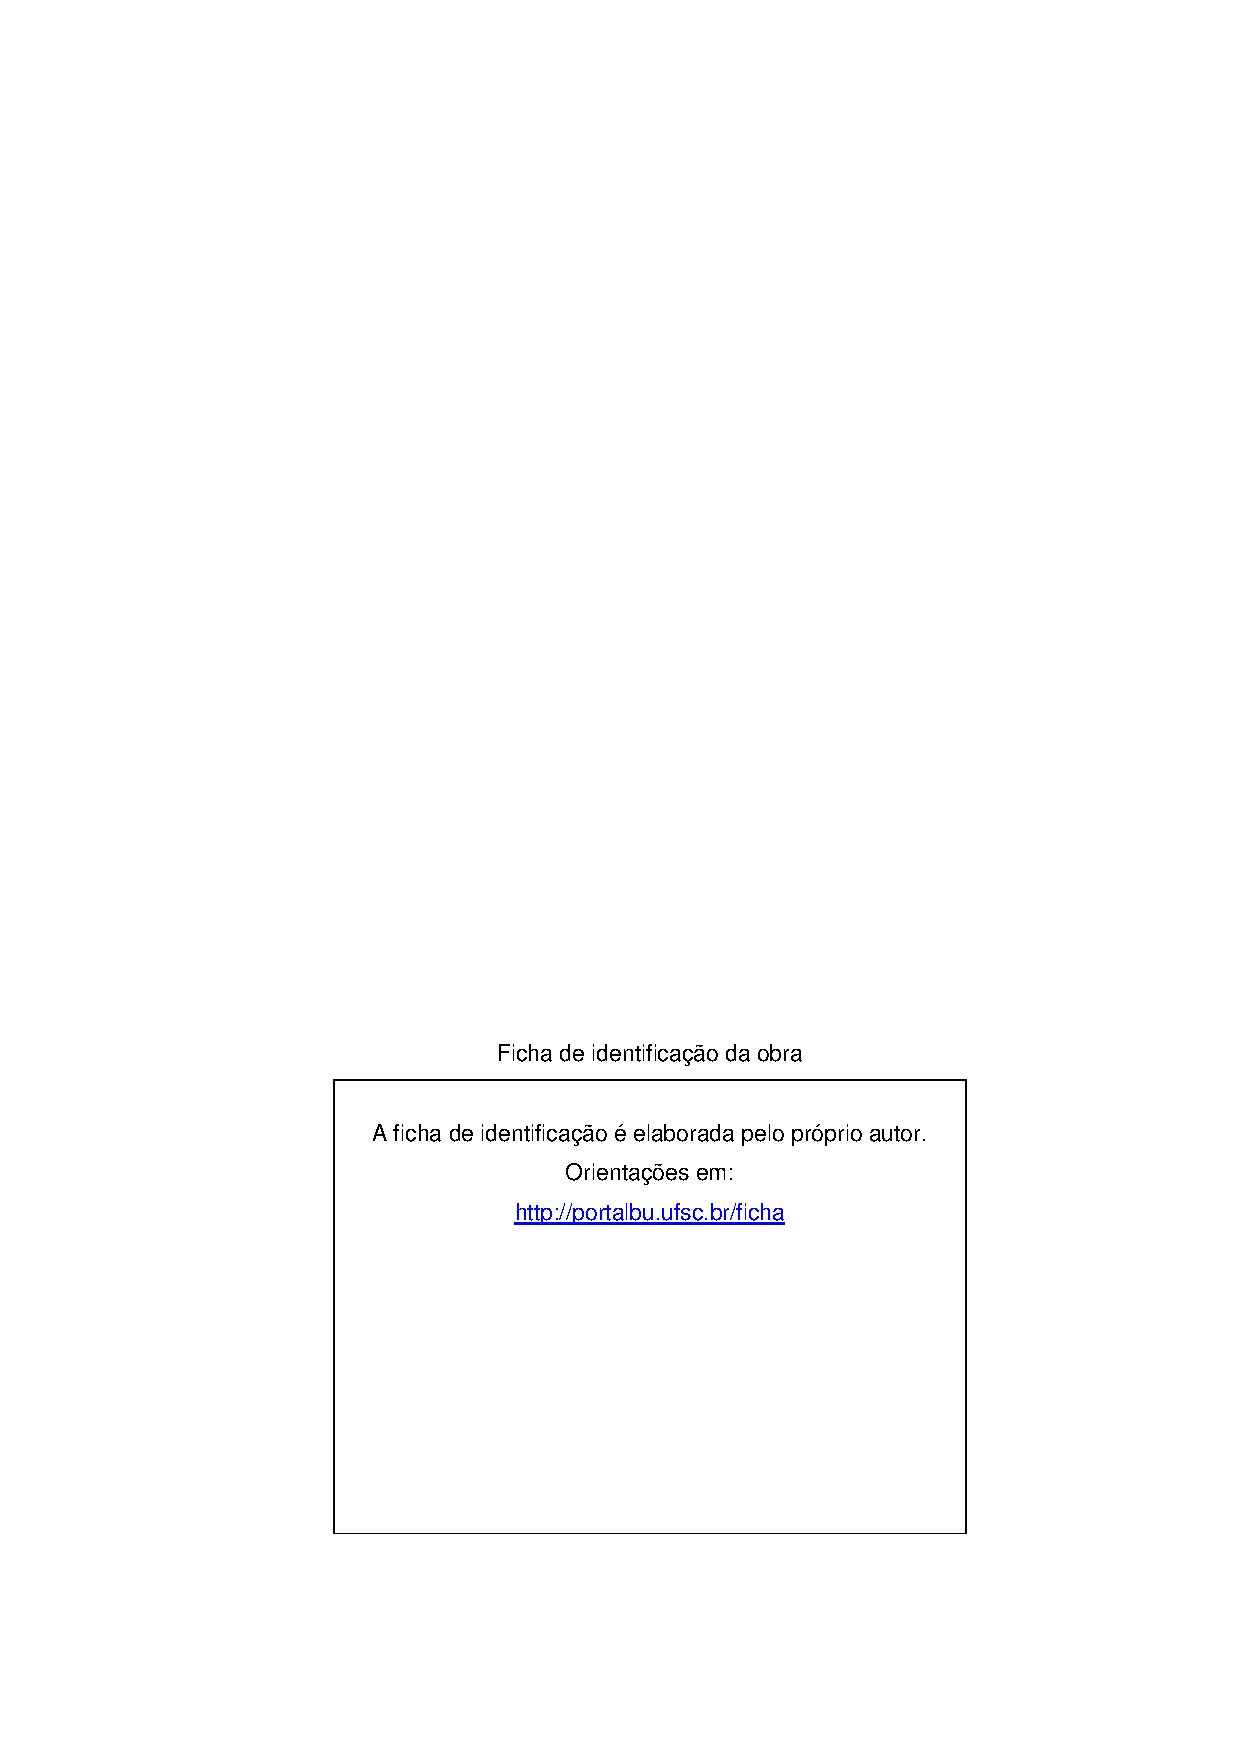
\includepdf{beforetext/Ficha_Catalografica.pdf}
%\end{fichacatalografica}
% ---

% ---
% Inserir folha de aprovação
% ---

%\begin{folhadeaprovacao}
%	\OnehalfSpacing
%	\centering
%	\imprimirautor\\%
%	\vspace*{10pt}		
%	\textbf{\imprimirtitulo}%
%	\ifnotempty{\imprimirsubtitulo}{:~\imprimirsubtitulo}\\%
%	%		\vspace*{31.5pt}%3\baselineskip
%	\vspace*{\baselineskip}
%	%\begin{minipage}{\textwidth}
%	% ~do~\imprimirprograma~do~\imprimircentro~da~\imprimirinstituicao~para~a~obtenção~do~título~de~\imprimirformacao.
%	Este~\imprimirtipotrabalho~foi julgado adequado para obtenção do Título de “\imprimirformacao” e aprovado em sua forma final pelo~\imprimirprograma. \\
%		\vspace*{\baselineskip}
%	\imprimirlocal, \imprimirdata. \\
%	\vspace*{2\baselineskip}
%	\assinatura{\OnehalfSpacing\imprimircoordenador \\ \imprimircoordenadorRotulo~do Curso}
%	\vspace*{2\baselineskip}
%	\textbf{Banca Examinadora:} \\
%	\vspace*{\baselineskip}
%	\assinatura{\OnehalfSpacing\imprimirorientador \\ \imprimirorientadorRotulo}
%	%\end{minipage}%
%	\vspace*{\baselineskip}
%	\assinatura{Prof.(a) xxxx, Dr(a).\\
%	Avaliador(a) \\
%	Instituição xxxx}
%
%	\vspace*{\baselineskip}
%	\assinatura{Prof.(a) xxxx, Dr(a).\\
%	Avaliador(a) \\
%	Instituição xxxx}


%\end{folhadeaprovacao}
% ---

% ---
% Dedicatória
% ---
%\begin{dedicatoria}
%	\vspace*{\fill}
%	\noindent
%	\begin{adjustwidth*}{}{5.5cm}     
%		Este trabalho é dedicado aos meus colegas de classe e aos meus queridos pais.
%	\end{adjustwidth*}
%\end{dedicatoria}
% ---

% ---
% Agradecimentos
% ---
%\begin{agradecimentos}
%	Inserir os agradecimentos aos colaboradores à execução do trabalho. 
	
%	Xxxxxxxxxxxxxxxxxxxxxxxxxxxxxxxxxxxxxxxxxxxxxxxxxxxxxxxxxxxxxxxxxxxxxx. 
%\end{agradecimentos}
% ---

% ---
% Epígrafe
% ---
%\begin{epigrafe}
%	\vspace*{\fill}
%	\begin{flushright}
%		\textit{``Texto da Epígrafe.\\
%			Citação relativa ao tema do trabalho.\\
%			É opcional. A epígrafe pode também aparecer\\
%			na abertura de cada seção ou capítulo.\\
%			Deve ser elaborada de acordo com a NBR 10520.''\\
%			(Autor da epígrafe, ano)}
%	\end{flushright}
%\end{epigrafe}
% ---

% ---
% RESUMOS
% ---

% resumo em português
\setlength{\absparsep}{18pt} % ajusta o espaçamento dos parágrafos do resumo
\begin{resumo}
	\SingleSpacing
    Com o uso de energia cada vez mais alto, surge a necessidade de se utilizar produtos cada vez mais eficientes. Compressores de refrigeradores são um dos grandes consumidores nas residências em todo mundo. Compressores lineares surgem como uma alternativa mais eficiente em relação aos compressores alternativos usados normalmente. Tendo isso em mente este trabalho implementa um modelo de compressor linear com os submodelos: elétrico, mecânico e termodinâmico, tendo como base um artigo científico. Após a implementação os submodelos foram validados e o modelo final comparado com um modelo consolidado para verificação. Além disso, uma análise de sensibilidade do modelo foi realizada a fim de entender melhor seu funcionamento. Os resultados obtidos mostraram que o modelo se comportou de forma similar ao do artigo base, apesar das modificações e adaptações feitas.
	
	\textbf{Palavras-chave}: Compressor linear. Modelo numérico. Refrigeração.
\end{resumo}

% resumo em inglês
%\begin{resumo}[Abstract]
%	\SingleSpacing
%	\begin{otherlanguage*}{english}
%		Resumo traduzido para outros idiomas, neste caso, inglês. Segue o formato do resumo feito na língua vernácula. As palavras-chave traduzidas, versão em língua estrangeira, são colocadas abaixo do texto precedidas pela expressão “Keywords”, separadas por ponto.
%		
%		\textbf{Keywords}: Keyword 1. Keyword 2. Keyword 3.
%	\end{otherlanguage*}
%\end{resumo}

%% resumo em francês 
%\begin{resumo}[Résumé]
% \begin{otherlanguage*}{french}
%    Il s'agit d'un résumé en français.
% 
%   \textbf{Mots-clés}: latex. abntex. publication de textes.
% \end{otherlanguage*}
%\end{resumo}
%
%% resumo em espanhol
%\begin{resumo}[Resumen]
% \begin{otherlanguage*}{spanish}
%   Este es el resumen en español.
%  
%   \textbf{Palabras clave}: latex. abntex. publicación de textos.
% \end{otherlanguage*}
%\end{resumo}
%% ---

%{%hidelinks
%	\hypersetup{hidelinks}
	% ---
	% inserir lista de ilustrações
	% ---
%	\pdfbookmark[0]{\listfigurename}{lof}
%	\listoffigures*
%	\cleardoublepage
	% ---
	
	% ---
	% inserir lista de quadros
	% ---
%	\pdfbookmark[0]{\listofquadrosname}{loq}
%	\listofquadros*
%	\cleardoublepage
	% ---
	
	% ---
	% inserir lista de tabelas
	% ---
%	\pdfbookmark[0]{\listtablename}{lot}
%	\listoftables*
%	\cleardoublepage
	% ---
	
	% ---
	% inserir lista de abreviaturas e siglas (devem ser declarados no preambulo)
	% ---
%	\imprimirlistadesiglas
	% ---
	
	% ---
	% inserir lista de símbolos (devem ser declarados no preambulo)
	% ---
%	\imprimirlistadesimbolos
	% ---
	
	% ---
	% inserir o sumario
	% ---
{
	\pdfbookmark[0]{\contentsname}{toc}
	\tableofcontents*
	\cleardoublepage
}	
%}%hidelinks
% ---
% ---

% ----------------------------------------------------------
% ELEMENTOS TEXTUAIS
% ----------------------------------------------------------
\textual

% ---
% 1 - Introdução
% ---
% ----------------------------------------------------------
\chapter{Visão Geral do Projeto}
% ----------------------------------------------------------

Nos dias de hoje, um refrigerador é um item indispensável em uma residência. Porém, a sua popularização é relativamente recente, datando da década de 1920, quando os refrigeradores elétricos passaram a ser acessíveis à população. No Brasil, o primeiro refrigerador nacional foi criado em Joinville, Santa Catarina, pela Consul, empresa criada no ano de 1950. Segundo Ono (2004), o primeiro modelo lançado foi o Q-300 em 1950, com um sistema de refrigeração por absorção, funcionando à base de querosene. Em 1956, a Consul também foi pioneira em trazer para o país o primeiro refrigerador elétrico, o Consul Elétrico.

Dada sua ampla utilização, os refrigeradores domésticos respondem por uma parcela significativa do consumo de energia. Juntamente com condicionadores de ar, esses dispositivos respondem por cerca de 17,2\% de todo o consumo de energia mundial (COULOMB et al., 2015). De acordo com  estimativas, existem cerca de 1,5 bilhões de refrigeradores domésticos em atividade no mundo \cite{refrigeration-ademe},.

Segundo o Anuário Estatístico de Energia Elétrica de 2020, da EMPRESA BRASILEIRA DE PESQUISA ENERGÉTICA (2020, p 48), o consumo de energia elétrica no setor residencial do Brasil passou de 131 190 GWh em 2015 para 142 781 GWh em 2019, o que representa um aumento de, aproximadamente, 8\% em quatro anos. Com o aumento do consumo de energia elétrica, surge a necessidade da fabricação de produtos que consumam menos energia e sejam mais eficientes, além de serem ecologicamente aceitáveis. Dentro dessa problemática, os compressores utilizados em refrigeradores domésticos são constantemente vistos como objetos de estudo em pesquisas relacionadas à eficiência energética.

Compressores alternativos, que geralmente realizam o processo de compressão de vapor através do movimento de um mecanismo biela-manivela, são os mais aplicados na refrigeração doméstica. Esse tipo de compressor possui diversos fatores que influenciam na perda de eficiência. Segundo Pérez-Segarra et al. (2005, apud SILVA E DUTRA, 2020, p. 5), as perdas de energia em um compressor podem ser divididas em três partes: (i) perdas elétricas causadas pela resistência ôhmica no motor, (ii) perdas mecânicas geradas pela fricção nos mancais e (iii) perdas termodinâmicas causadas pelas irreversibilidades durante o processo de compressão do gás.

Compressores lineares são uma alternativa interessante aos compressores alternativos. O modelo linear não utiliza o movimento rotativo dos motores elétricos tradicionais, mas usa um motor elétrico linear para promover o movimento alternado do pistão. O funcionamento de um motor linear é semelhante, porém o estator, que é onde as bobinas estão, não é circundado ao rotor, nesse caso conhecido como cursor. Em outras palavras, o cursor se move axialmente em relação ao estator. Complementando o que foi dito, Liang (2017) descreve:

\begin{citacao}
Compressor linear não possui mecanismo biela-manivela quando comparado com compressores convencionais alternativos. Isso permite maior eficiência,  ausência de óleo lubrificante, menor custo e menor tamanho quando comparado com modelos comuns usados em sistemas de refrigeração por compressão de vapor.(LIANG, 2017, p. 253, tradução nossa)
\end{citacao}

Seguindo a ideia de Liang (2017), um compressor linear não possui o mecanismo de biela-manivela, então o atrito com os mancais é desconsiderado, além disso, não existe a necessidade de óleo lubrificante, tornando assim o sistema mais atrativo em relação ao cuidado com o meio ambiente. Dessa forma, o desenvolvimento da tecnologia dos compressores lineares se torna pertinente, visto que cumpre as necessidades de ser um produto energeticamente mais eficiente e menos agressivo ao meio ambiente.

Compressores lineares já são empregados em alguns refrigeradores domésticos disponíveis no mercado. Desde 2002 a empresa sul-coreana LG tem comercializado este tipo de compressor para sistemas de refrigeração, tendo licenciado a tecnologia da empresa Sunpower. No Brasil, a Embraco desenvolveu a tecnologia Wisemotion, que é uma linha de compressores lineares que não utiliza óleo, tendo sido lançada no mercado em 2014. Tronbini (2016) explica algumas qualidades oferecidas pela tecnologia:

\begin{citacao}
A tecnologia atende níveis de eficiência que podem chegar a 20\% de economia de energia quando comparada aos compressores de alta eficiência mais vendidos mundialmente. “Outra vantagem do Wisemotion é proporcionar uma melhor conservação dos alimentos, por manter a temperatura interna do refrigerador estável”, aponta a empresa. O desenvolvimento do compressor levou dez anos e envolveu 100 profissionais de Pesquisa e Desenvolvimento, tendo gerado 80 patentes globalmente. (TRONBINI, 2016, online)
\end{citacao}

A partir das informações apresentadas, é visível a inovação que os compressores lineares trazem em relação aos alternativos convencionais, se consolidando como uma alternativa tecnológica para aumentar a eficiência energética de refrigeradores domésticos. Entretanto, sendo esta uma tecnologia recente, ainda apresenta grandes oportunidades de melhoria. Um exemplo disso é a proposta de Silva e Dutra (2020) de otimizar a trajetória do pistão ao longo do processo de compressão, o que tem potencial de aumentar a eficiência termodinâmica em até 25,9\% e a eficiência volumétrica em até 6,1\% em condições típicas de refrigeração doméstica. Dentro deste contexto, espera-se neste trabalho estudar e implementar o modelo eletromecânico de um compressor linear a fim de permitir avaliar futuramente as perdas elétricas e mecânicas de um compressor com trajetória de pistão otimizada.


%As orientações aqui apresentadas são baseadas em um conjunto de normas elaboradas pela \gls{ABNT}. Além das normas técnicas, a Biblioteca também elaborou uma série de tutoriais, guias, \textit{templates} os quais estão disponíveis em seu site, no endereço \url{http://portal.bu.ufsc.br/normalizacao/}.

%Paralelamente ao uso deste \textit{template} recomenda-se que seja utilizado o \textbf{Tutorial de Trabalhos Acadêmicos} (disponível neste link \url{https://repositorio.ufsc.br/handle/123456789/180829}) e/ou que o discente \textbf{participe das capacitações oferecidas da Biblioteca Universitária da UFSC}.

%Este \textit{template} está configurado apenas para a impressão utilizando o anverso das folhas, caso você queira imprimir usando a frente e o verso, acrescente a opção \textit{openright} e mude de \textit{oneside} para \textit{twoside} nas configurações da classe \textit{abntex2} no início do arquivo principal \textit{main.tex} \cite{abntex2classe}.

%Os trabalhos de conclusão de curso (TCC) de graduação e de especialização não são entregues em formato impresso na Biblioteca Universitária. Porém, sua versão PDF pode ser disponibilizada no Repositório Institucional, consulte seu curso sobre os procedimentos adotados para a entrega. 

% ----------------------------------------------------------
%Uma nota de rodapé, já tem seu estilo automático com o comando \texttt{$\backslash$footnote}\footnote{As notas de rodapé possuem fonte tamanho 10. O alinhamento das linhas da nota de rodapé deve ser abaixo da primeira letra da primeira palavra da nota de modo dar destaque ao expoente.}.


% ----------------------------------------------------------
\section{Objetivos}
% ----------------------------------------------------------

Para desenvolver este trabalho, propõe-se os seguintes objetivos.

% ----------------------------------------------------------
\subsection{Objetivo Geral}
% ----------------------------------------------------------

Implementar um modelo numérico do sistema eletromecânico de um compressor linear.

% ----------------------------------------------------------
\subsection{Objetivos Específicos}
% ----------------------------------------------------------

\begin{itemize}
\item
Implementar e validar um submodelo elétrico de motor linear.
\item
Implementar e validar um submodelo mecânico para o movimento do pistão.
\item
Implementar um submodelo termodinâmico simplificado para o ciclo de compressão.
\item
Acoplar os submodelos elétrico, mecânico e termodinâmico em um único modelo.
\item
Comparar  os resultados do modelo implementado com dados da literatura.
\item
Avaliar a influência de diferentes parâmetros sobre o funcionamento do compressor.
\end{itemize}
% ---

% ---
% 2 - Capítulo 2
% ---
% ----------------------------------------------------------
\chapter{FUNDAMENTAÇÃO TEÓRICA}\label{cap:desenvolvimento}

Para obter resultados de um trabalho é necessário entender o problema, seus componentes, as ferramentas à disposição e saber unir todos os pontos. A primeira parte da fundamentação teórica serve para criar uma base para o entendimento dos componentes: sistema de refrigeração e compressor linear. A segunda parte, e último tópico, explica o método de resolução numérico.

\section{SISTEMAS DE REFRIGERAÇÃO}
% ----------------------------------------------------------

Refrigeradores domésticos geralmente utilizam o ciclo de compressão de vapor com um gás refrigerante, por exemplo, R-134a, que permanece confinado no sistema. O ciclo padrão de compressão é representado na Figura \ref{fig:Fig_1}, onde é possível identificar os seus quatro componentes básicos: condensador, dispositivo de expansão, evaporador e compressor.

\begin{figure}[htb]
	\caption{\label{fig:Fig_1}Ciclo padrão de refrigeração por compressão de vapor.}
	\begin{center}
		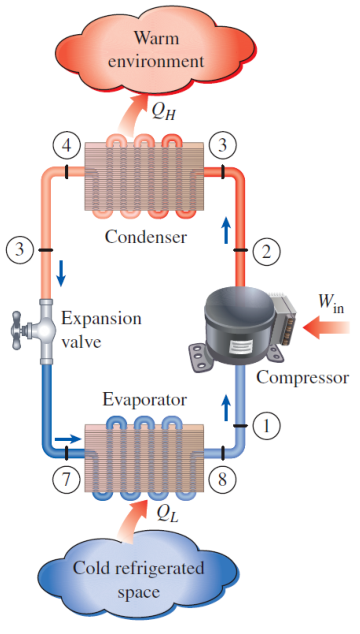
\includegraphics[scale=0.65]{images/refrigerador.png}
	\end{center}
	\fonte{Çengel e Boles (2005)}
\end{figure}

 No ciclo padrão de compressão de vapor ilustrado na Figura \ref{fig:Fig_1}, um fluido na fase gasosa a baixa pressão entra no compressor, que o comprime e superaquece. Em seguida, o fluido de trabalho, a alta temperatura e pressão, passa por um condensador, onde troca calor com o ambiente, vindo a condensar. Após a condensação, o fluido entra num dispositivo de expansão, onde sua pressão e temperatura são reduzidas. Após a expansão, o fluido bifásico passa pelo evaporador, onde absorve calor do espaço refrigerado. Por fim, o fluido retorna para o compressor, onde o ciclo se reinicia.

\section{COMPRESSOR LINEAR}

Normalmente, os compressores de refrigeradores domésticos são alternativos, os quais são classificados como compressores de deslocamento positivo por proporcionarem um aumento de pressão do gás de trabalho a partir da diminuição do seu volume. A câmara de compressão é formada por um conjunto pistão-cilindro, sendo que o movimento alternativo do pistão é geralmente realizado por um sistema biela-manivela. O funcionamento dos compressores lineares é bastante similar. Entretanto, o movimento alternativo do pistão é realizado por um motor linear..
De acordo com Oliveira (2014) é possível encontrar quatro componentes básicos em um compressor linear (Figura \ref{fig:Fig_2}): bobina elétrica, magneto, pistão e molas. A partir de uma tensão elétrica oscilante, a bobina gera um campo eletromagnético variável que exerce uma força sobre o magneto, ocasionando a movimentação conjunta do magneto e do pistão, que estão acoplados. O pistão se move dentro do cilindro e realiza a compressão e expansão do fluido de trabalho. As molas são responsáveis por armazenar energia cinética para que o sistema possa trabalhar em ressonância.


\begin{figure}[htb]
	\caption{\label{fig:Fig_2}Esquemático básico de um compressor linear.}
	\begin{center}
		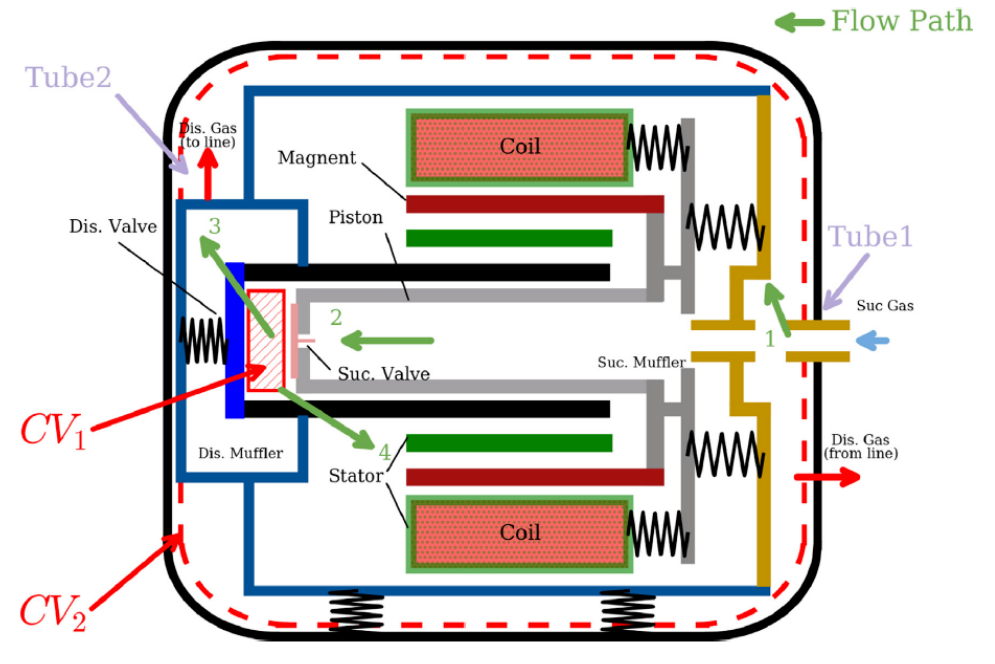
\includegraphics[scale=0.50]{images/compressor.png}
	\end{center}
	\fonte{Zhang et al. (2020)}
\end{figure}

Ainda analisando a Figura \ref{fig:Fig_2}, o caminho percorrido pelo fluido pode ser indicado pelas setas.O fluido de trabalho entra na carcaça do compressor, a baixa pressão, passa por dentro do pistão e é succionada para dentro da câmara de compressão pela válvula de sucção. A válvula de sucção é dita automática, pois abre e fecha de acordo com as diferenças de pressão entre a câmara de compressão e o ambiente interno do compressor. Com o fluido na câmara de compressão e a válvula de sucção fechada o fluido é comprimido durante o movimento ascendente do pistão. A compressão acontece até que a pressão dentro da câmara de compressão seja levemente superior à pressão de descarga, o que ocasiona a abertura da válvula de descarga e a liberação do gás para a linha de descarga.



\section{MÉTODO RUNGE KUTTA DE 4ª ORDEM}

O método de Runge-Kutta (RK) é utilizado para resolver equações diferenciais ordinárias (EDO) com problema de valor inicial (PVI). Assim como Zhang et al. (2020a), este trabalho adotará o método de RK de quarta ordem para resolver as equações governantes do problema. Como as equações descritas neste trabalho são de segunda ordem, foi necessário transformá-las em um sistema de duas equações de primeira ordem para aplicar o método. Sendo assim, a explicação se restringe a uma EDO genérica de primeira ordem.
Seja y'a derivada primeira de y, onde y é uma função de t.Valores iniciais de y' e y são conhecidos e mostrados nas Equações \ref{eq:y_linha} e \ref{eq:y_comum}:



\begin{equation}\label{eq:y_linha}
y' = f(t,y),
\end{equation}


\begin{equation}\label{eq:y_comum}
y(t_0)=y_0,
\end{equation}


A solução que o método Runge-Kutta propõe para a EDO a cada intervalo discreto de tempo é dado pelas Equações \ref{eq:y} e \ref{eq:t}:




\begin{equation}\label{eq:y}
y_{n+1}=y_n+ \frac{h}{6}(K1+2K2+2K3+K4),
\end{equation}


\begin{equation}\label{eq:t}
t_{n+1}=t_n+h,
\end{equation}
onde a letra h é o passo de tempo do método, e n um número inteiro que representa o índice relacionado a um determinado instante de tempo. As funções K1, K2, K3 e K4 são definidos nas Equações \ref{eq:k1}, \ref{eq:k2}, \ref{eq:k3} e \ref{eq:k4}:


\begin{equation}\label{eq:k1}
K1=f(t_n,y_n),
\end{equation}

\begin{equation}\label{eq:k2}
K2=f(t_n+ \frac{h}{2},y_n+\frac{h}{2}K1),
\end{equation}

\begin{equation}\label{eq:k3}
K3=f(t_n+ \frac{h}{2},y_n+\frac{h}{2}K2),
\end{equation}

\begin{equation}\label{eq:k4}
K4 = f(t_n + h, y_n + hK3 ).
\end{equation}



% ---

% ---
% 3 - Capítulo 3
% ---
% ----------------------------------------------------------
\chapter{METODOLOGIA}
% ----------------------------------------------------------


Este trabalho foi baseado na pesquisa de Zhang et al. (2020a), cujos autores resolvem um modelo numérico de compressor linear completo (sistemas elétrico, mecânico,  termodinâmico) utilizando o software PDSim (BELL et al., 2020). Neste trabalho optou-se por desenvolver o submodelo em uma linguagem de programação amplamente utilizada a fim de futuramente acoplá-los a um software de simulação termodinâmico existente implementado em C++.

Nesta seção serão apresentadas as etapas de implementação do algoritmo para a integração dos submodelos desenvolvidos e os submodelos desenvolvidos: mecânico, elétrico e termodinâmico. Para que a implementação numérica fosse possível, este estudo se deu com uso do software Matlab e da biblioteca termodinâmica CoolProp, desenvolvida por Bell et al. (2014).

Os resultados obtidos por Zhang et al. (2020a) serão utilizados como comparação para o modelo desenvolvido. Entretanto, deve-se salientar que o submodelo termodinâmico de Zhang et al. (2020a) inclui efeitos de vazamento, transferência de calor e movimento de válvulas, por exemplo. Tais efeitos tornam a simulação mais verossímil quando comparada com um ciclo de compressão ideal. Levando isso em conta, espera-se que haja alguma divergência nos resultados quando as comparações envolverem os submodelos termodinâmicos.

\section{GEOMETRIA E DADOS DO COMPRESSOR}

Com a geometria definida é possível encontrar dados importantes, como volume da câmara de compressão, área do pistão, valor da massa efetiva e dados sobre o circuito elétrico do motor. Tais dados serão usados para a resolução dos submodelos mecânico e elétrico, e estão dispostos na Tabela \ref{tab:Tab_1} :







\begin{table}[htb]
	\ABNTEXfontereduzida
	\caption{\label{tab:Tab_1} Dados da geometria e motor para o compressor}
	\begin{center}
	\begin{tabular}{p{5.0cm}p{1.5cm}p{2cm}p{2.5cm}}
		\toprule
		\textbf{Parâmetro} &  \textbf{Símbolo}      & \textbf{Valor} & \textbf{Unidade}    \\ \midrule
	Diâmetro do pistão                 & $D_p$              & 26,5              & $mm$                                      \\
		Massa do pistão                    & $m_p$          & 0,632            & $kg$                                        \\
		Massa das molas                    & $m_s$          & 0,164             & $kg$                                       \\
		Constante de rigidez das molas     & $k_s$          & 45,66             & $Nmm^{-1}$                                  \\
        Fator de motor                     & $\alpha$       & 75             & $NA^{-1}$                                        \\ 
		Resistência elétrica do motor      & $\Omega$       & 15,7             & $\Omega$                                     \\ 
		Indutância do motor                & $L$            & 450             & $mH$                                            \\ \bottomrule
	\end{tabular}
	\end{center}
	\fonte{Adaptado de Zhang et al. (2020)}
\end{table}

O dado da capacitância não foi apresentado em Zhang et al. (2020a). Esse dado foi calculado utilizando a Equação 9, com os valores de R, L e as curvas de deslocamento e corrente fornecidas nos resultados de Zhang et al. (2020a). Para um dado instante de tempo é possível encontrar os valores para todos os elementos da Equação 9 menos a capacitância, assim isolando-a e encontrando seu valor. Neste caso o valor encontrado foi de C = 35F.

\section{CONDIÇÕES DE OPERAÇÃO}

A condição de operação pode ser descrita pelos parâmetros listados na Tabela \ref{tab:Tab_2}. Tais dados foram retirados da Tabela 3.1 de Zhang et al. (2020), com exceção do valor da razão de pressões, PR. 



\begin{table}[htb]
	\ABNTEXfontereduzida
	\caption{\label{tab:Tab_2}Condições de operação para o compressor}
	\begin{center}
	\begin{tabular}{p{5.0cm}p{1.5cm}p{2cm}p{2.5cm}}
		\toprule
		\textbf{Parâmetro} &  \textbf{Símbolo}      & \textbf{Valor} & \textbf{Unidade}    \\ \midrule
	    Fluido de trabalho              & -              & R134a        & -                                      \\
		Pressão de sucção               & $P_{suc}$          & 111,81   & $Pa$                                        \\
		Temperatura de Sucção           & $T_{suc}$          & 8,08     & $°C$                                       \\
        Razão de pressões               & $PR$       & 4,9              & -                                        \\ 
		Frequência de operação          & $f$       & 60                & $Hz$                                     \\  \bottomrule
	\end{tabular}
	\end{center}
	\fonte{Adaptado de Zhang et al. (2020)}
\end{table}


O valor da razão de pressões de Zhang et al. (2020a) descrito em seu artigo é 5,5. Porém, analisando os resultados de Zhang et al (2020a), que apresenta valores para pressão na câmara de compressão, e com ajuda da plataforma online WebPlotDigitalizer (ROHATGI, 2020), é possível perceber que pressão descarga é igual a, aproximadamente, 4,9 vezes maior que a pressão de sucção.

%\begin{figure}[htb]
%	\caption{\label{fig:zhang_pressao}Gráfico do resultado de Zhang et al. (2020a) em regime permanente da pressão no cilindro em função do tempo.}
%	\begin{center}
%		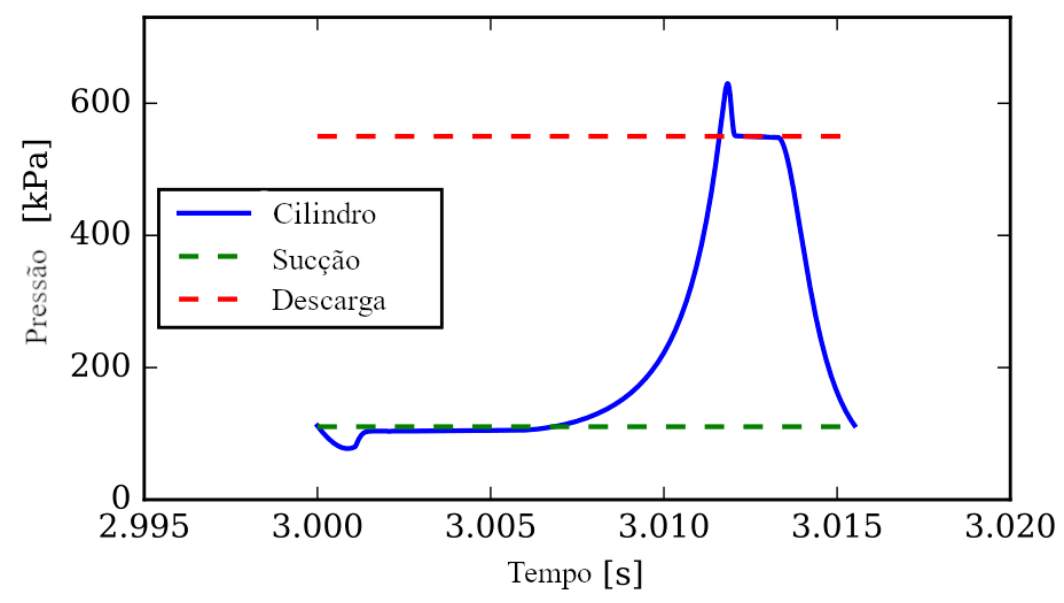
\includegraphics[scale=0.4]{images/pressao_zhang.png}
%	\end{center}
%	\fonte{Adaptado de Zhang et al. (2020)}
%\end{figure}

%Ainda analisando a Figura \ref{fig:zhang_pressao}, o dado apresentado pelo autor para PR = 5,5 não condiz com o apresentado em seu resultado. Por esse motivo se fez necessário e justificável realizar esta alteração nos dados da referência.

\section{MODELO NUMÉRICO}

A modelagem numérica de um problema representa, de forma simplificada, o processo de algum fenômeno. No caso de um compressor linear, é preciso levar em conta três submodelos: (i) o elétrico, que determina a força eletromagnética agindo sobre o magneto a partir de dados de tensão de entrada e movimento do pistão; (ii) o mecânico, que determina a posição do pistão a partir de todas as excitações sofridas; e (iii) o termodinâmico, que calcula o esforço exercido pelo gás comprimido sobre o pistão.


\subsection{Submodelo elétrico}

É prática comum na literatura representar o motor de um compressor linear como um circuito RLC (Zhang et al., 2020a; Bijanzad et al., 2020a), consistindo de um resistor, um indutor e um capacitor ligados em série com uma fonte de tensão (Figura \ref{fig:circuito-eletrico}). Resultados obtidos por Zhang et al. (2020b) foram inclusive utilizados para validar este modelo.

\begin{figure}[htb]
	\caption{\label{fig:circuito-eletrico} Diagrama do circuito elétrico usado em compressores lineares.}
	\begin{center}
		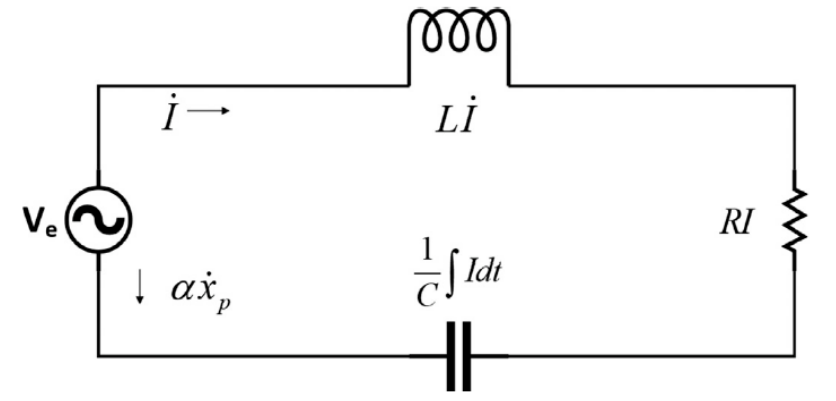
\includegraphics[scale=0.65]{images/circuito.png}
	\end{center}
	\fonte{Adaptado de Zhang et al. (2021)}
\end{figure}

Na Figura \ref{fig:circuito-eletrico}, a variável I, representa a corrente elétrica , R a resistência ,L a indutância, C a capacitância ,t o tempo ,Ve a tensão alternada e uemft é a força eletromotriz inversa, que é proveniente da própria Lei de Faraday aplicada. Essa força ocorre normalmente em motores elétricos devido ao movimento relativo do magneto, que gera uma diferença de potencial. O equacionamento do circuito pode ser obtido a partir das leis de Kirchhoff como mostrado na Equação \ref{eq:eletrico}: 




\begin{equation}\label{eq:eletrico}
V_e-u_{emf}(t)= LI'+RI+\frac{1}{C} \int I \,dt ,
\end{equation}


onde $u_{emf}(t)$ é definido a partir da Lei de Faraday:




\begin{equation}\label{eq:uemf}
u_{emf}(t)=Blx'_p= x'p.
\end{equation}


Nesta Equação \ref{eq:uemf}, B é a densidade magnética das bobinas, l o tamanho do condutor, e , que é o produto de B e l, é o fator de motor. Além desses parâmetros, a velocidade instantânea do pistão entra no cálculo como x'p.
A potência elétrica consumida pelo motor pode ser calculada a partir da Equação 11:

\begin{equation}\label{eq:uemf}
W_{e} = f \int_{0}^{1/f} V_eI(t)\,dt
\end{equation}


\subsection{Submodelo mecânico}

No caso do modelo mecânico, o mecanismo é tratado como um sistema massa-mola-amortecedor. Nesse caso, o diagrama de corpo livre do pistão pode ser observado na Figura \ref{fig:forcas-atuando}. A variável $P(t)$ representa a pressão na câmara de compressão, $P_{shell}$ é a pressão de sucção existente no ambiente interno do compressor, $A_p$ é a área da seção transversal do pistão, $k_s$ é a constante de rigidez da mola, $c_{fri}$ é o coeficiente de fricção, $I(t)$ representa a corrente elétrica instantânea,  é o fator de motor, e $x_p$,$x^{'} _p$ e $x{''} _p$ representam o deslocamento, velocidade e aceleração do pistão, respectivamente. Reunindo todos esses termos e aplicando a segunda Lei de Newton obtém-se:


\begin{figure}[htb]
	\caption{\label{fig:forcas-atuando} Representação das forças atuando no pistão.}
	\begin{center}
		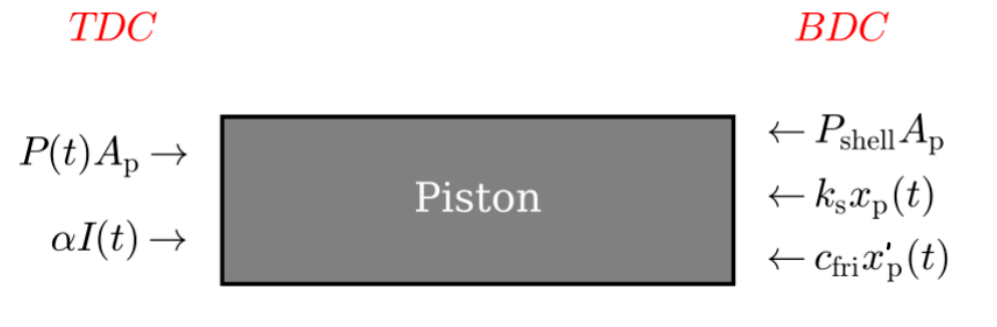
\includegraphics[scale=0.65]{images/pistao.png}
	\end{center}
	\fonte{Adaptado de Zhang et al. (2020a)}
\end{figure}

\begin{equation}\label{eq:mecanico}
m_{eff}x''_p + c_{fri}x'_p+ k_{s}x_p + (P_shell - P(t))A_p = \alpha I(t) 
\end{equation}

A Equação \ref{eq:mecanico} representa a equação de movimento do pistão, onde $m_{eff}$ é a massa efetiva do sistema.

%Na Figura \ref{fig:dados_ref} é possível ver o pistão dentro do cilindro. TDC significa \textit{Top Dead Center}, do inglês, BDC é o \textit{Bottom Dead Center}. $X_m$é a posição sobre a qual o sistema oscila harmonicamente, esse valor pode variar conforme o carregamento dinâmico no pistão é alterado. $X_0$ é a distância fixa entre a placa da válvula de descarga e o topo do pistão quando não há nenhum carregamento dinâmico atuando no pistão. 


%\begin{figure}[htb]
%	\caption{\label{fig:dados_ref}Descrição de dados para referência no cálculo do pistão.}
%	\begin{center}
%		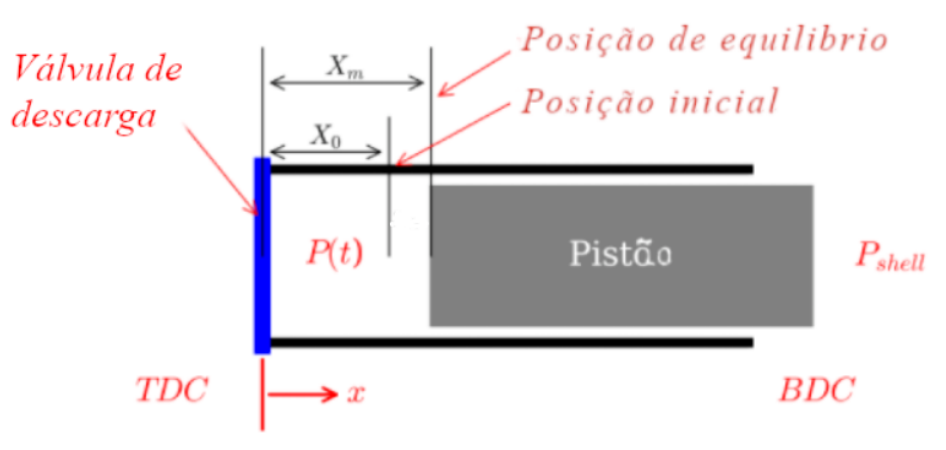
\includegraphics[scale=0.65]{images/pistao_02.png}
%	\end{center}
%	\fonte{Adaptado de Zhang et al. (2021)}
%\end{figure}

%O volume na câmara de compressão é calculado pela  Equação \ref{eq:volume}:


%\begin{equation}\label{eq:volume}
% V= x_{rp}A_p,
%\end{equation}

%onde $x_{rp}$ é definido na Equação \ref{eq:xrp}: 

%\begin{equation}\label{eq:xrp}
%x_{rp} = x_p + X_0,
%\end{equation}
%e $x_p$ é a posição de deslocamento do pistão em relação a $X0$.
%Em algumas situações específicas, observou-se que o carregamento de pressão sobre o pistão poderia ocasionar valores negativos de xrp,fazendo com que o volume da câmara de compressão fosse negativo e gerando erros na simulação. Essa condição foi observada durante o transiente inicial do compressor e em determinadas condições de operação nas quais a posição de equilíbrio fica muito próxima da placa de válvulas. A fim de evitar erros na simulação, decidiu-se implementar uma força de mola fictícia ao pistão  quando ele passa de um determinado volume mínimo. Essa força pode ser vista na Equação 15:

%\begin{equation}\label{eq:f_virt}
%F_{a} = k_{virtual}max( 0 , 0.0004 - X_0 - x_p),
%\end{equation}
%onde kvirtual foi adotado igual a 5,106 N/m. A força $Fa$, atua no sentido positivo do eixo x, tendendo a afastar o pistão da placa de válvulas.  Ainda com relação a Equação \ref{eq:f_virt}, é necessário deixar bem claro que essa adaptação só passa a ocorrer caso o pistão esteja a uma distância inferior a 0,0004 m da placa de válvulas.

A potência mecânica, transmitida pelo motor ao pistão pode ser calculada como:


\begin{equation}\label{eq:f_virt}
W_{m} = f \int_{0}^{1/f} I(t)x'_p(t) \,dt
\end{equation}

\subsection{Submodelo termodinâmico}

Este trabalho tem como foco a implementação dos submodelos elétrico e mecânico, embora seja necessário um submodelo termodinâmico para prever o carregamento de pressão sobre o pistão. Logo, optou-se pelo submodelo termodinâmico mais simples possível, ou seja, o ciclo ideal de compressão de vapor foi considerado, sendo compreendido por processos de expansão e compressão isentrópicos e processos de sucção e descarga isobáricos (Figura \ref{fig:grafico_pv}).


\begin{figure}[htb]
	\caption{\label{fig:grafico_pv}Diagrama Pressão-Volume do ciclo ideal de compressão de vapor com a explicação de cada ciclo e o sentido.}
	\begin{center}
		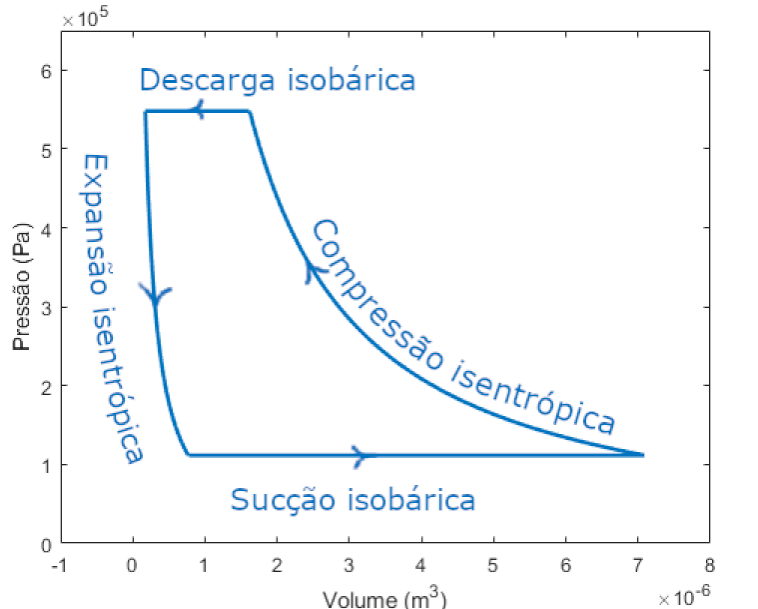
\includegraphics[scale=0.50]{images/termodinamico.png}
	\end{center}
	\fonte{Autor (2021)}
\end{figure}

A potência termodinâmica, $W_t$, pode ser calculada a partir da integração do diagrama pressão-volume. Assim, as eficiências elétrica e mecânica podem ser obtidas a partir do acoplamento de todos os submodelos. A eficiência elétrica, $\eta_e$, representa a razão entre a potência mecânica, $W_m$, e a potência elétrica, $W_e$, enquanto a eficiência mecânica, $\eta_m$, representa a razão entre a potência termodinâmica e a potência mecânica.

\section{RESOLUÇÃO DAS EQUAÇÕES}

O problema apresenta três submodelos, e dois deles envolvem equações diferenciais ordinárias de segunda ordem, representada pelas Equações 9 e 12, sendo, respectivamente, os submodelos elétrico e mecânico. Essas equações foram resolvidas utilizando o método de Runge Kutta de 4ª ordem.
Na Figura \ref{fig:fluxograma}, é possível observar todas as etapas da metodologia de resolução adotada. 

\begin{figure}[htb]
	\caption{\label{fig:fluxograma}Fluxograma da linha de cálculo do algoritmo.}
	\begin{center}
		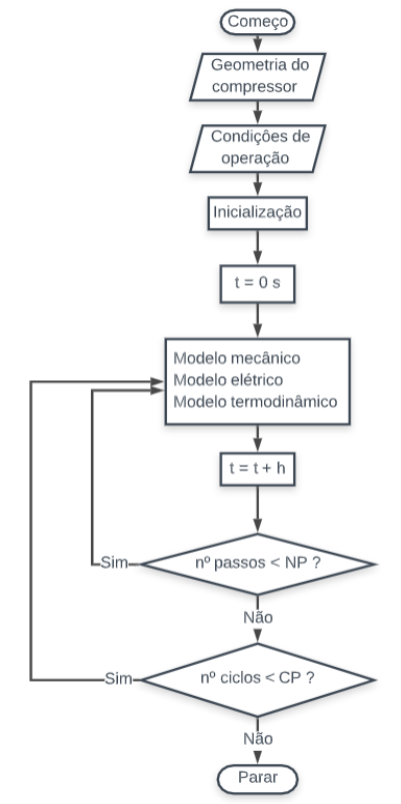
\includegraphics[scale=0.65]{images/modelo_geral.png}
	\end{center}
	\fonte{Autor (2021)}
\end{figure}


A Figura \ref{fig:fluxograma} mostra a lógica adotada, onde “CP” é o número total de passos que cada ciclo tem e “NP”  é o número total de passos, caso o valor não tenha atingido o número total de de passos do ciclo ele retorna ao looping, caso esses valores sejam iguais, o código avança para o próximo ciclo, assim até completar o número de ciclos desejados. No caso deste trabalho o número de passos, CP, é 1000 e o número de ciclos, NP, 100.
A única variável de entrada é o valor da tensão, que foi definida a partir dos resultados de Zhang et al. (2020), sendo mostrada na Equação \ref{eq:ve} : 


\begin{equation}\label{eq:ve}
V_e(t)=220cos(2\pi60t)
\end{equation}

\vfill \break


É possível observar na Equação \ref{eq:ve} que a frequência de oscilação é igual a 60 Hz e uma tensão alternada de 220 V, em outras palavras, é uma tensão nominal comum numa residência.

%A Figura \ref{fig:rk} é um esquemático do acontece dentro do método de Runge-Kutta aplicado, cada submodelo é dependente do outro. A cada loop feito representa um passo de tempo h fixo, a duração do ciclo é definida pela frequência dada T =1/f   e o passo é definido h=T/NC onde NC é um número pré-definido pelo usuário. A quantidade de ciclos feitos também é um dado que o usuário pode escolher.


%\begin{figure}[htb]
%	\caption{\label{fig:rk}Esquema de resolução dentro do método de Runge-Kutta}
%	\begin{center}
%		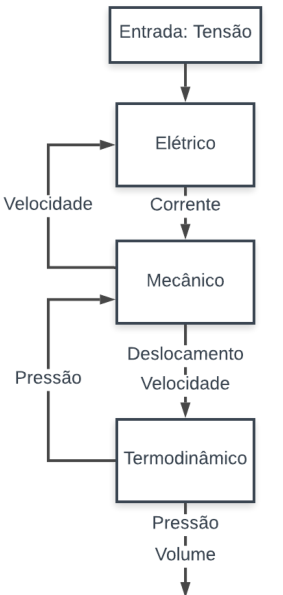
\includegraphics[scale=0.70]{images/modelo_rk.png}
%	\end{center}
%	\fonte{Autor (2021)}
%\end{figure}

%Percebe-se pela Figura \ref{fig:rk} que cada submodelo é dependente do outro: o elétrico depende da velocidade do pistão, pois ocorre o efeito da Lei de Faraday. O mecânico depende da pressão na câmara de compressão do termodinâmico e da corrente do elétrico. O termodinâmico depende da velocidade e deslocamento do pistão do mecânico. E dessa forma os submodelos se integram e formam o modelo desenvolvido.

% ---

% ---
% 4 - Resultados
% ---
%\phantompart
% ----------------------------------------------------------
\chapter{RESULTADOS}
% ----------------------------------------------------------


Esta seção tratará dos resultados obtidos, com a implementação da metodologia proposta no Capítulo 3, adaptações que precisaram ser feitas, e observações com relação ao modelo desenvolvido por Zhang et al. (2020a).
Antes da implementação integral de todos os submodelos, cada submodelo, mecânico e elétrico,  foi validado de forma separada. Dessa forma, foi possível ter um controle maior sobre cada operação. Cada submodelo foi validado com os resultados obtidos de Zhang et al. (2020a). Além dessa validação independente, uma validação da junção do modelo mecânico e elétrico, mas sem o termodinâmico, foi feita.
A implementação integral dos três submodelos apresentados não é uma validação, tendo em vista que os mesmo submodelos que Zhang et al. (2020a) utilizou não foram todos aplicados neste trabalho. Contudo, é possível fazer uma comparação dos resultados para perceber se há coerência no resultado final.   
	
\section{VALIDAÇÃO DO SUBMODELO ELÉTRICO}
				
Para a validação deste submodelo foi resolvida a Equação \ref{eq:eletrico} pelo método de Runge-Kutta de quarta ordem. Dados de entrada nesse modelo são os valores de $R$, $L$, $C$, $V_e$ e por fim $u_{emf}$, com isso a resolução do sistema retorna o valor de $I(t)$ em função do tempo.

Observações foram feitas com relação ao valor do fator de motor,  = 75 $NA{-1}$, dado na Tabela \ref{tab:Tab_1}, e foi percebido uma certa inconsistência no valor fornecido. 
%Pode-se ver na Figura \ref{fig:comp_e_75} uma comparação entre os resultados de Zhang et al. (2020a) e aqueles obtidos no presente trabalho. 
Convém ressaltar que foi feita uma verificação do método Runge-Kutta comparando-o com uma rotina pré-existente no Matlab. 



% \begin{figure}[htb]
%	\caption{\label{fig:comp_e_75}Comparação das curvas para o submodelo elétrico tendo como referência Zhang et al. (2020a). Discrepância entre os resultados para  = 75 NA-1.}
%	\begin{center}
%		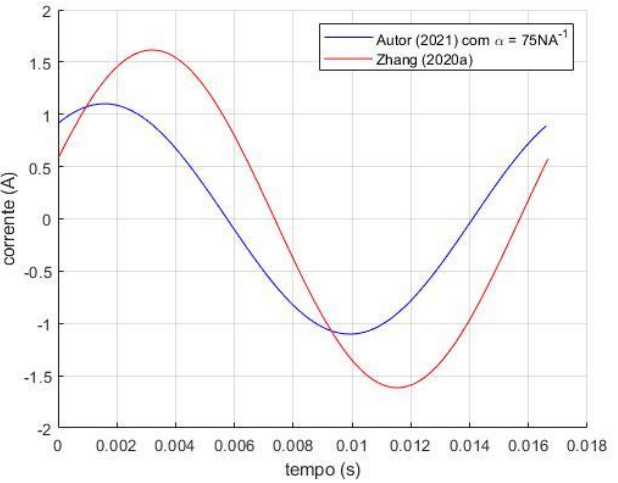
\includegraphics[scale=0.6]{images/e_75.png}
%	\end{center}
%	\fonte{Autor (2021)}
%\end{figure}

Para resolver esse problema, tentou-se contatar sem sucesso os autores do referido trabalho a fim de verificar um possível erro tipográfico no artigo. Posteriormente, vários valores de  foram testados como entrada, até que se percebeu um padrão na movimentação da curva resultante. Dessa forma, foi encontrado um valor em que a resposta se justapõe muito bem na curva de referência. No caso, o valor encontrado foi de  = 35 $NA^{-1}$, e a nova comparação pode ser vista na Figura \ref{fig:comp_e_35}. Sabe-se que o valor encontrado pode não ser correto, e com isso não ter um resultado correto, porém adotou-se esse valor para que futuramente esse dado possa ser encontrado 




 \begin{figure}[h]
	\caption{\label{fig:comp_e_35}Comparação das curvas para o submodelo elétrico tendo como referência Zhang et al. (2020a). Concordância entre os resultados para  = 35 NA-1.}
	\begin{center}
		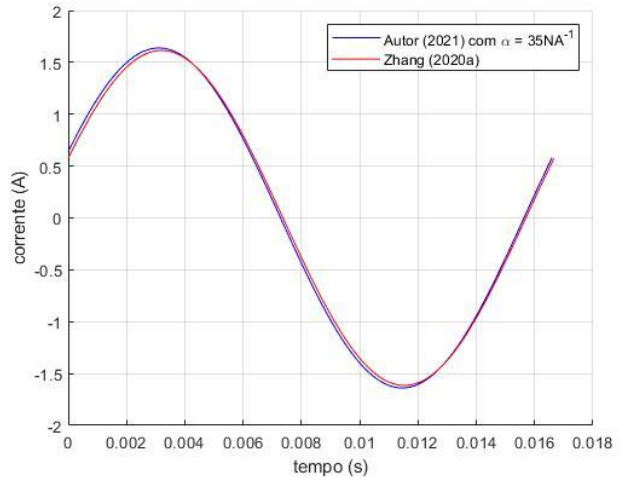
\includegraphics[scale=0.55]{images/e_35.png}
	\end{center}
	\fonte{Autor (2021)}
\end{figure}

A curva da Figura \ref{fig:comp_e_35}, apresenta os dois resultados praticamente iguais. Com esse resultado, assume-se que esse submodelo fornece resultados que são coerentes, visto que se aproximou do resultado de Zhang et al. (2020a), apesar da inconsistência encontrada no fator de motor. 
\vfill

\section{VALIDAÇÃO DO SUBMODELO MECÂNICO}

Para a validação do submodelo mecânico foi resolvida a Equação \ref{eq:mecanico} pelo método de Runge-Kutta de quarta ordem. Dados de entrada nesse modelo são os valores de $m_{eff}$, $k_s$, $c_{fri}$, $P_{shell}$, $P(t)$, $A_p$, $\alpha$ e por fim $I(t)$, com isso a resolução do sistema retorna o valor de $x_p(t)$ em função do tempo.

Na etapa da validação do submodelo mecânico, assim como o submodelo elétrico,  Zhang et al. (2020a) não divulgaram o valor do coeficiente de fricção, $c_{fri}$. Por consequência, dados sobre coeficiente de fricção em compressores lineares foram pesquisados. Na tese de doutorado de Bradshaw (2012), sobre um modelo miniatura de um compressor linear para arrefecimento de eletrônicos, o autor comenta que utiliza valores entre 0,1 e 0,3 kg/s em seu trabalho.

Dessa forma, foram adotados como possíveis valores: 0,1, 0,2 e 0,3 kg/s. Ao aplicar esses valores no código não houve diferença perceptível em relação ao resultado, porém percebeu-se que quanto maior o valor de $c_{fri}$ mais rápido a simulação atinge uma condição de regime periódico. Além disso, embora os autores tenham fornecido as massas do pistão e das molas, eles não indicaram a massa móvel efetiva do sistema. Como uma primeira tentativa, optou-se por calcular a massa efetiva como $m_{eff}=m_p+1/3m_s$, onde $m_p$ é a massa do pistão e ms é a massa das molas, conforme sugerido por Rao (2018). %A Figura \ref{fig:m_13} é o resultado do submodelo mecânico para $m_{eff}=m_p+1/3m_s$, e é representada num gráfico de deslocamento por tempo. 

 % \begin{figure}[htb]
%	\caption{\label{fig:m_13}Comparação do deslocamento por tempo para com o submodelo mecânico, tendo massa efetiva do sistema igual a $m_{eff}=m_p+1/3 ; m_s=0.6867$ kg com o resultado de Zhang et al. (2020).}
%	\begin{center}
%		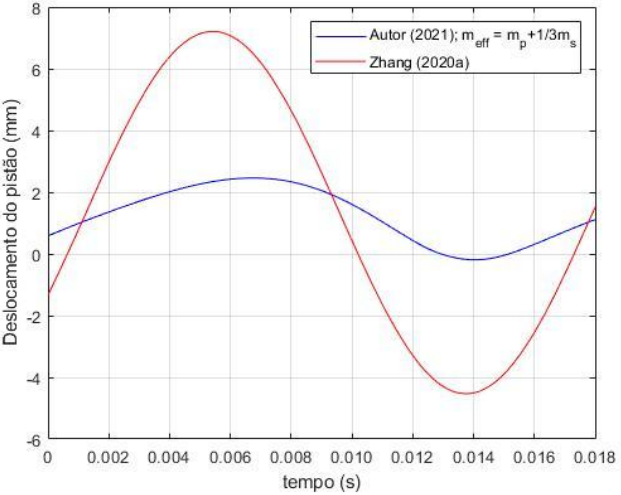
\includegraphics[scale=0.65]{images/m_13.png}
%	\end{center}
%	\fonte{Autor (2021)}
%\end{figure}


%Analisando a Figura \ref{fig:m_13} é possível observar a comparação entre deslocamento no pistão para meff=mp+1/3ms e a referência. A amplitude do deslocamento é relativamente menor que de Zhang et al. (2020a), não sendo um valor aceitável para uma validação.Dentre as alternativas para contornar esse problema, a que mais fez sentido, foi ajustar o valor da massa efetiva, visto que não foi fornecida. Dessa forma escolheu-se a como a massa efetiva a própria massa do pistão, porém os resultados também não foram aceitáveis, a Figura \ref{fig:comp_m_orig2} mostra o resultado da simulação com $m_{eff}=m_p =0,632 kg$.
 
	
% \begin{figure}[htb]
%    \caption{\label{fig:comp_m_orig2}Comparação das curvas para com o submodelo mecânico, tendo massa efetiva do sistema igual a $m_{eff}=0,632 kg$}
%    \begin{center}
%	    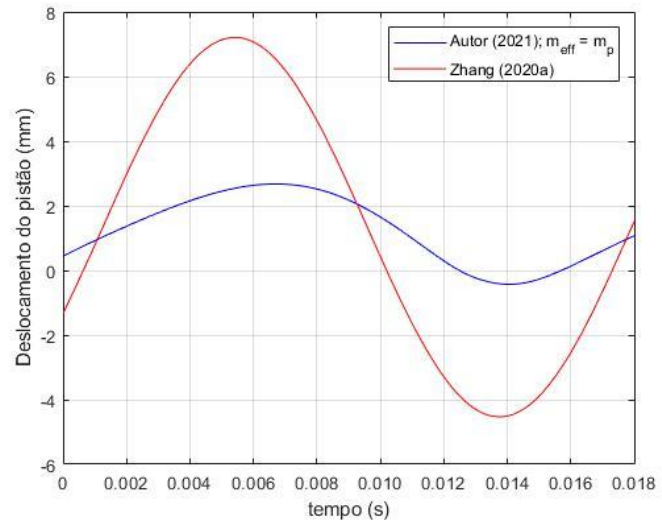
\includegraphics[scale=0.65]{images/m_p.png}
%    \end{center}
%    \fonte{Autor (2021)}
%\end{figure}


%A Figura \ref{fig:comp_m_orig2} assim como a \ref{fig:m_13} comparam o deslocamento do pistão em relação a Zhang et al. (2020a). Os dois resultados tiveram resultados próximos pelo motivo da massa efetiva não variar significativamente. De certa forma, era esperado um resultado não muito diferente em relação ao anterior. 
Tendo resultados para $m_{eff}$ não aceitáveis com o método dito, decidiu-se encontrar uma massa efetiva que aproximasse os resultados. Então, foi adotado $m_{eff}$ =0,400 kg. É entendido que este é um valor irreal, pois a massa mínima esperada seria o peso do pistão, contudo isso é um ponto a ser melhorado em trabalhos futuros. Os resultados de deslocamento do pistão são comparados na Figura \ref{fig:comp_m_04}, que apresenta amplitudes aparentemente iguais, porém com fases um pouco diferentes. Supõe-se que esta defasagem seja um efeito combinado de incertezas associadas tanto à massa efetiva quanto ao coeficiente de fricção. Supõe-se que um ajuste melhor das curvas possa ser obtido variando estes dois parâmetros em um procedimento de otimização. Porém, considera-se que os resultados atuais já são suficientes para atender os objetivos do presente trabalho, sendo, portanto, adotados como valores de referência daqui pra frente.

 \begin{figure}[htb]
	\caption{\label{fig:comp_m_04}Comparação das curvas para com o submodelo mecânico, tendo massa efetiva do sistema igual a $me_{eff}=0,400kg$.}
	\begin{center}
		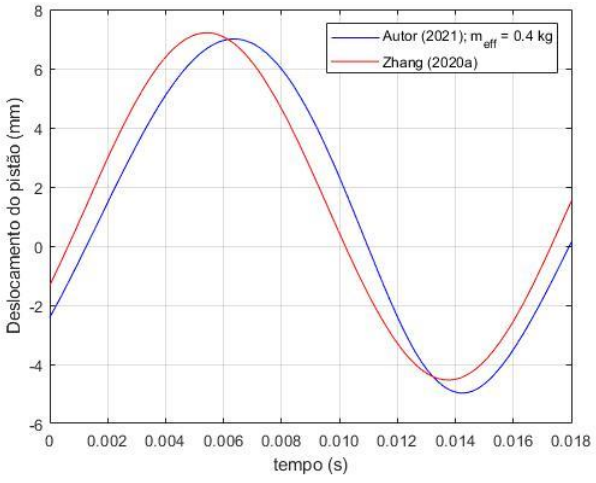
\includegraphics[scale=0.65]{images/m_04.png}
	\end{center}
	\fonte{Autor (2021)}
\end{figure}

%\section{VALIDAÇÃO DO MODELO ELETROMECÂNICO ACOPLADO}

%Com as validações apresentadas nas Seções 4.1 e 4.2, pode-se partir para validação da união dos dois submodelos. O resultado do deslocamento do pistão em função do tempo pode ser visto na Figura 15, onde é mostrada a oscilação resultante do pistão em regime periódico.


 %\begin{figure}[htb]
%	\caption{\label{fig:comp_e_m}Comparação do resultado que mostra o deslocamento pelo tempo da união dos submodelos mecânico e elétrico em relação a Zhang et al (2020a).}
%	\begin{center}
%		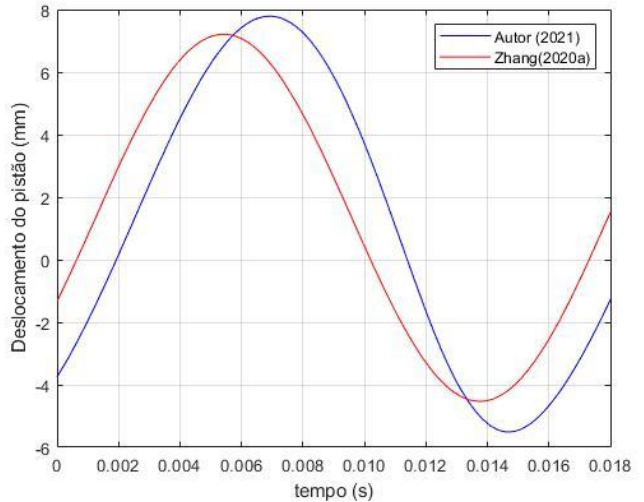
\includegraphics[scale=0.55]{images/e_m.png}
%	\end{center}
%	\fonte{\cite{bradshaw}}
%\end{figure}


%Analisando o acoplamento dos dois submodelos em relação ao deslocamento na Figura \ref{fig:comp_e_m}, é possível perceber uma pequena diferença em relação a validação do submodelo mecânico, isso acontece pelo fato de que no submodelo mecânico, os dados da corrente elétrica foram retirados dos resultados de Zhang et al. (2020a), não sendo afetados pela velocidade do pistão com a força eletromotriz inversa. Enquanto no acoplamento dos submodelos, a corrente já é calculada tendo como parâmetro de entrada a velocidade do pistão. Dessa forma, como já havia uma pequena discrepância nos resultados obtidos no submodelo mecânico, esse erro pode ter se propagado para a união dos submodelos.
%Para entender melhor o efeito percebido na Figura \ref{fig:comp_e_m}, os dados da corrente do modelo eletromecânico e do submodelo mecânico foram comparados em um gráfico pelo tempo. Tais dados são mostrados na Figura \ref{fig:comp_acopl}. 


 %\begin{figure}[htb]
%	\caption{\label{fig:comp_acopl}Comparação das curvas da corrente pelo tempo do submodelo eletromecânico acoplado com o submodelo mecânico.}
%	\begin{center}
%		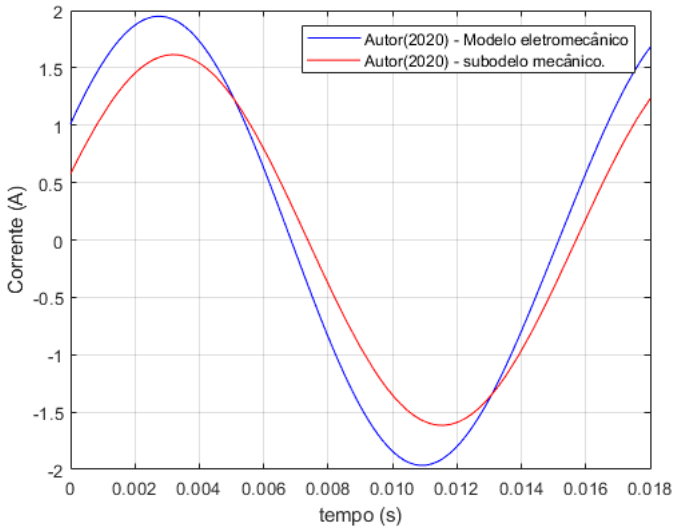
\includegraphics[scale=0.55]{images/c_e_m.png}
%	\end{center}
%	\fonte{\cite{bradshaw}}
%\end{figure}

%Percebe-se, na Figura \ref{fig:comp_acopl}, que existe uma variação da corrente entre os dois modelos, isto se deve pelo fato de no modelo eletrodinâmico a velocidade do pistão interferir na corrente com a força eletromotriz inversa, e no mecânico a corrente usada é o resultado de Zhang et al. (2020a), não sendo afetada pela velocidade do pistão.

\section{ACOPLAMENTO DO MODELO ELETROMECÂNICO COM O TERMODINÂMICO}

Toda a teoria apresentada, discutida e de certa forma validada foi necessária para ser aplicada nesta seção. Como comentado anteriormente, devido ao fato do modelo de Zhang et al. (2020a) e este desenvolvido não aplicarem os mesmos submodelos, não faz sentido validar o modelo aqui desenvolvido. Tendo isso em vista, ao invés de uma validação foi feita uma comparação com o modelo de Zhang et al. (2020a). Embora não se espere que os resultados obtidos sejam exatamente iguais, é possível compará-los a fim de verificar  a coerência física.
Esta seção mostra o resultado do acoplamento do modelo eletromecânico com o ciclo ideal de compressão do vapor. O resultado do deslocamento pelo tempo pode ser visto na Figura \ref{fig:comp_desloc}. Esses dados representam o deslocamento no centésimo ciclo, já em regime periódico. O deslocamento, na abscissa, dos dois modelos se apresenta próximo. 


 \begin{figure}[htb]
	\caption{\label{fig:comp_desloc}Comparação do resultado do deslocamento do pistão entre o modelo desenvolvido neste trabalho e ao modelo de Zhang et al (2020a).}
	\begin{center}
		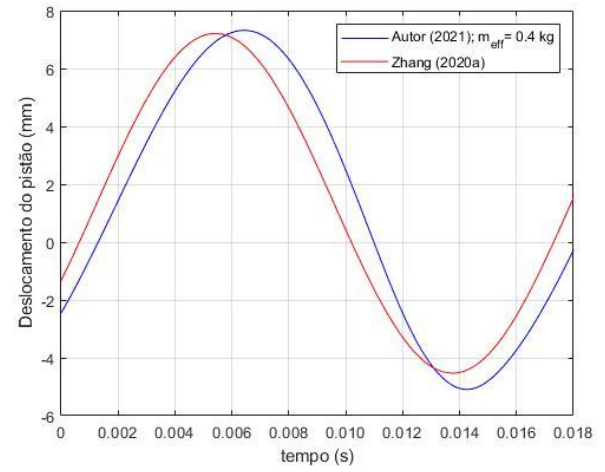
\includegraphics[scale=0.60]{images/e_m_t.png}
	\end{center}
	\fonte{Autor (2021)}
\end{figure}


%A Figura \ref{fig:comp_pres} compara a pressão na câmara de compressão do modelo desenvolvido com o resultado de Zhang et al. (2020) para o centésimo ciclo. Na Figura \ref{fig:comp_pres} ainda é possível observar os efeitos de vazamentos e a dinâmica de válvulas  não aplicadas no modelo.

% \begin{figure}[htb]
%	\caption{\label{fig:comp_pres}Pressão em função do tempo na câmara de compressão em comparação com a de Zhang et al. (2020).}
%	\begin{center}
%		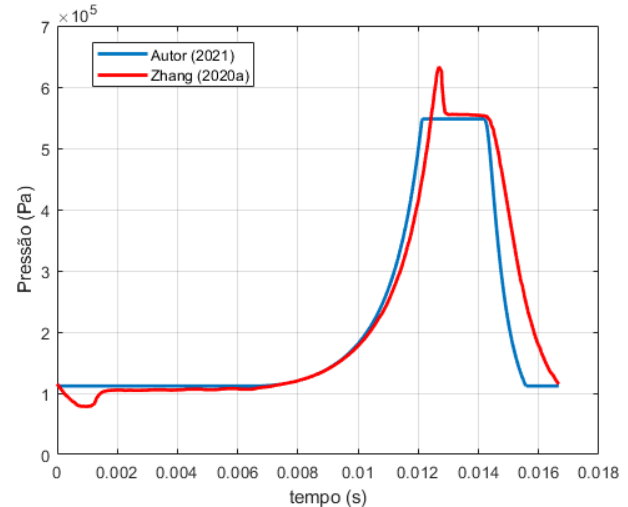
\includegraphics[scale=0.60]{images/pressao_zhang_02.png}
%	\end{center}
%	\fonte{Autor (2021)}
%\end{figure}


%A Figura \ref{fig:comp_pres} apresenta a pressão variando em função do tempo. Com isso, percebe-se, no modelo desenvolvido, que no instante 0,012 s a válvula de descarga é aberta mantendo a pressão constante até aproximadamente o instante 0,014. De fato, isso condiz com a Figura \ref{fig:comp_desloc}, no instante  0,012 s o pistão está chegando no TDC, comprimindo o fluido de trabalho. No instante 0,014 o deslocamento começa no sentido contrário, o que faz com que a válvula de descarga se feche e dessa forma diminuindo bruscamente a pressão.



 %\begin{figure}[htb]
%	\caption{\label{fig:comp_elet}Comparação do resultado mostrado em função das correntes pelo tempo entre o modelo desenvolvido neste trabalho e ao modelo de Zhang et al (2020a).}
%	\begin{center}
%		\includegraphics[scale=0.60]{images/c_c_zhang.png}
%	\end{center}
%	\fonte{Autor (2021)}
%\end{figure}

%A Figura \ref{fig:comp_elet} apresenta a comparação do resultado da corrente com o resultado de Zhang et al. (2020) para o centésimo ciclo. Comparando a Figura \ref{fig:comp_elet} com a do modelo eletromecânico, Figura 16, observou-se uma menor amplitude da corrente. Esse fato pode ser explicado pelo modelo eletromecânico comparado usar os dados da pressão de Zhang et al. (2020), enquanto o modelo da Figura \ref{fig:comp_elet} usa o ciclo ideal de compressão.

%É importante ressaltar que durante esta simulação observou-se que a força fictícia $F_a$, dada pela equação 7, foi ativada mesmo quando o sistema atinge a condição periódica. Isso se deve ao fato de que o carregamento dinâmico de pressão sobre o pistão foi alterado em relação ao resultado apresentado por Zhang et al. (2020a), uma vez que os submodelos termodinâmicos não são exatamente iguais.
\vfill


\section{ANÁLISE DA SENSIBILIDADE DO MODELO} 

Após as validações e comparações, nesta seção serão mostradas algumas análises feitas, entre elas: eficiências mecânica e elétrica em função da variação da razão de pressão, PR, variação das potências mecânica e elétrica em função da razão de pressão e uma análise da transmissibilidade do pistão.
Na Figura \ref{fig:comp_PR_efic}, é possível observar como as eficiências variam de acordo com a razão de pressão. Observa-se que a eficiência mecânica tende a aumentar enquanto que a eficiência elétrica sofre menos variações. Percebe-se também que quando PR = 3,6, existe um aumento brusco de eficiência mecânica acompanhado de uma redução significativa de eficiência elétrica, porém, não foi entendido o porquê desse comportamento. Simulações adicionais, além dos pontos mostrados na Figura \ref{fig:comp_PR_efic}, realizadas com PR próxima a 3,6 indicam que realmente existe um ponto ótimo de eficiência elétrica nessa região.  


 \begin{figure}[htb]
	\caption{\label{fig:comp_PR_efic} Análise de diferentes razões de pressões e seu efeito nas eficiências.}
	\begin{center}
		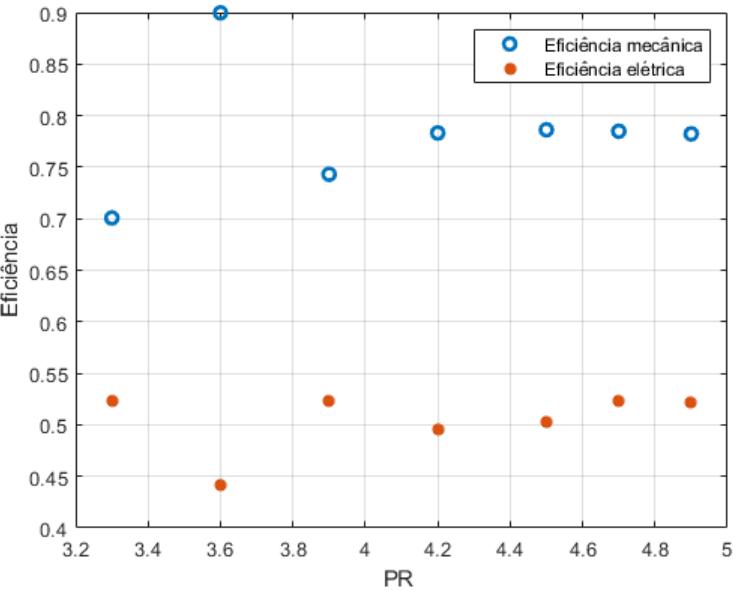
\includegraphics[scale=0.50]{images/efic.png}
	\end{center}
	\fonte{Autor (2021)}
\end{figure}




Na Figura \ref{fig:comp_PR_pot} encontram-se as potências em cada etapa: potência elétrica, potência mecânica, e potência termodinâmica. Percebe-se que, de fato, a potência elétrica consumida quando PR = 3,6 assume um mínimo e que mesmo que a potência mecânica também seja menor, a queda brusca da potência elétrica justifica o aumento da eficiência elétrica. Sendo assim, em trabalhos futuros será conveniente entender as razões que levam a essa condição de potência elétrica. 

 \begin{figure}[htb]
	\caption{\label{fig:comp_PR_pot}Análise do efeito da variação da razão de pressões nas potências elétrica, mecânica e termodinâmica.}
	\begin{center}
		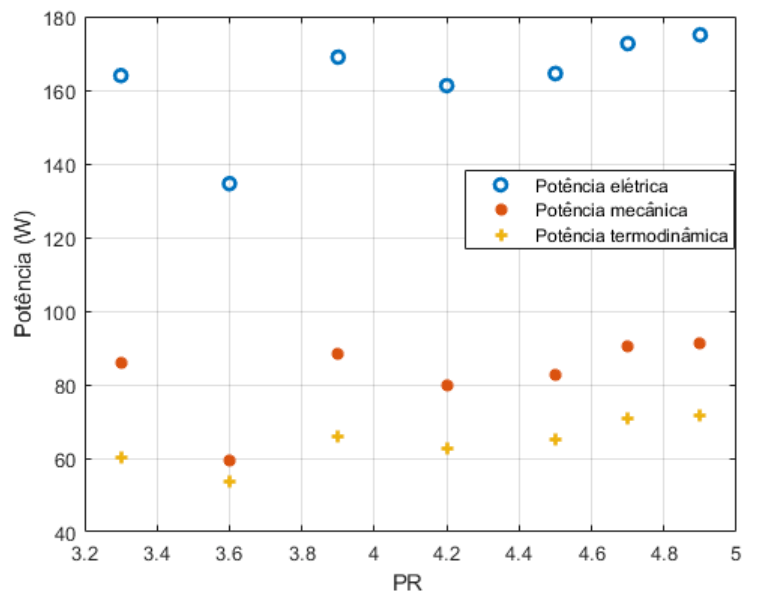
\includegraphics[scale=0.50]{images/pote.png}
	\end{center}
	\fonte{Autor (2021)}
\end{figure}

\nocite{anuario}
\nocite{bijanzada}
\nocite{bijanzadb}
\nocite{bradshaw}
\nocite{coolprop}
\nocite{coulomb}
\nocite{liang}
\nocite{oliveira}
\nocite{ono}
\nocite{pdsim}
\nocite{rao}
\nocite{refrigeration-ademe}
\nocite{silva}
\nocite{webplot}
\nocite{zhanga}
\nocite{zhangb}

% ---

% ---
% 4 - Conclusão
% ---
%\phantompart
% ----------------------------------------------------------
\chapter{Conclusão}
% ----------------------------------------------------------

O presente estudo procurou modelar um compressor linear tendo como base um artigo científico disponível na literatura. Buscou-se dividir o modelo nos submodelos elétrico, mecânico e termodinâmico, fazendo implementações individuais e, posteriormente, realizando a sua integração completa. Assim, com resultados do artigo base e resultados do modelo desenvolvido pôde-se fazer uma comparação e uma avaliação entre os dois.
Durante o desenvolvimento deste trabalho, foram identificados alguns empecilhos e discrepâncias. Por exemplo, alguns parâmetros necessários à simulação não foram fornecidos no artigo de referência e outros apresentaram inconsistência em relação aos resultados apresentados no próprio artigo. Ainda assim, buscou-se uma forma coerente e lógica de resolver cada um desses problemas.

A comparação chave foi o deslocamento do pistão ao longo do tempo, mostrada em cada validação e comparação, visto que, predizer onde o pistão estará é um problema pertinente e não é tão simples como em um compressor alternativo convencional, no qual o movimento é geralmente imposto por um mecanismo biela-manivela. Os resultados de deslocamento do pistão obtidos indicam uma coerência física do modelo desenvolvido, embora algumas melhorias ainda precisam ser implementadas. Uma análise da influência da razão de pressão sobre as potências e eficiências também foi realizada a fim de ilustrar o uso do modelo. Essa análise indicou a existência de um ponto ótimo de eficiência elétrica quando a razão de pressão se aproxima de 3,6, o que é plenamente justificado pelo decaimento brusco da potência elétrica. As razões dessa queda de potência não foram identificadas e permanecem como uma questão a ser verificada no futuro.

Como sugestões para trabalhos futuros, destaca-se:
\begin{itemize}
    \item Melhorar a estimativa do coeficiente de fricção;
    \item Desenvolver uma metodologia para verificar quando a simulação atinge a condição periódica;
    \item Acoplar os modelos elétrico e mecânico implementados ao modelo termodinâmico de Silva e Dutra (2020);
    \item Modelar sistemas de controle de movimento de pistão, existentes em compressores lineares reais, a fim de evitar o choque do pistão contra a placa de válvulas mesmo em condições adversas de operação;
    \item Identificar as razões que levam a potência elétrica a reduzir drasticamente em razões de pressão próximas de 3,6.
\end{itemize}

Tendo o objetivo de modelar um compressor linear, este trabalho utilizou conceitos de diferentes disciplinas do curso de Engenharia Aeroespacial, como circuitos elétricos, vibrações mecânicas, ciclos termodinâmicos e métodos numéricos de resolução de equações diferenciais, além de toda a capacidade lógica e de análise que um problema de engenharia requer. Em outras palavras, cada etapa de formação foi necessária para este momento.

% ---

% ----------------------------------------------------------
% ELEMENTOS PÓS-TEXTUAIS
% ----------------------------------------------------------
\postextual
% ----------------------------------------------------------

% ----------------------------------------------------------
% Referências bibliográficas
% ----------------------------------------------------------
\begingroup
    \SingleSpacing\printbibliography[title=REFERÊNCIAS]
\endgroup

% ----------------------------------------------------------
% Glossário
% ----------------------------------------------------------
%
% Consulte o manual da classe abntex2 para orientações sobre o glossário.
%
%\glossary

% ----------------------------------------------------------
% Apêndices
% ----------------------------------------------------------

% ---
% Inicia os apêndices
% ---
%\begin{apendicesenv}
%	\partapendices* 
%	% ----------------------------------------------------------
\chapter{Descrição}
% ----------------------------------------------------------

Textos elaborados pelo autor, a fim de completar a sua argumentação. Deve ser precedido da palavra APÊNDICE, identificada por letras maiúsculas consecutivas, travessão e pelo respectivo título. Utilizam-se letras maiúsculas dobradas quando esgotadas as letras do alfabeto. 

\begin{quadro}[htb]
	\centering
	\caption{\label{qua:Quadro_2}Modelo A.}	
\begin{tabular}{|l|l|}
\hline
xxxx              & yyyyyyyyyyyyyyy    \\
\hline
xxxx              & yyyyyyyyyyyyyyy    \\
\hline
xxxx              & yyyyyyyyyyyyyyy    \\
\hline
xxxx              & yyyyyyyyyyyyyyy    \\
\hline
xxxx              & yyyyyyyyyyyyyyy    \\
\hline
xxxx              & yyyyyyyyyyyyyyy    \\
\hline
xxxx              & yyyyyyyyyyyyyyy    \\
\hline
rrrrrrrrrrrrrrrrr & eeeeeeeeeeeeeeeee  \\
\hline
xxxx              & yyyyyyyyyyyyyyy    \\
\hline
xxxx              & yyyyyyyyyyyyyyy    \\
\hline
rrrrrrrrrrrrrrrrr & eeeeeeeeeeeeeeeee  \\
\hline
xxxx              & yyyyyyyyyyyyyyy    \\
\hline
                  & ttttttttttttttttt  \\
\hline
rrrrrrrrrrrrrrrrr & eeeeeeeeeeeeeeeee  \\
\hline
ttttttttttttt     &                    \\
\hline
rrrrrrrrrrrrrrrrr & eeeeeeeeeeeeeeeee  \\
\hline
rrrrrrrrrrrrrrrrr & eeeeeeeeeeeeeeeee  \\
\hline
                  & gggggggggggggggggg \\
\hline
rrrrrrrrrrrrrrrrr & eeeeeeeeeeeeeeeee  \\
\hline
rrrrrrrrrrrrrrrrr & eeeeeeeeeeeeeeeee  \\
\hline
rrrrrrrrrrrrrrrrr & eeeeeeeeeeeeeeeee  \\
\hline
rrrrrrrrrrrrrrrrr & eeeeeeeeeeeeeeeee  \\
\hline
\end{tabular}
\fonte{Elaborada pelo autor (2016).}
\end{quadro}
%\end{apendicesenv}
% ---


% ----------------------------------------------------------
% Anexos
% ----------------------------------------------------------

% ---
% Inicia os anexos
% ---
%\begin{anexosenv}
%	\partanexos*
%	% ----------------------------------------------------------
\chapter{Descrição}
% ----------------------------------------------------------

São documentos não elaborados pelo autor que servem como fundamentação (mapas, leis, estatutos). Deve ser precedido da palavra ANEXO, identificada por letras maiúsculas consecutivas, travessão e pelo respectivo título. Utilizam-se letras maiúsculas dobradas quando esgotadas as letras do alfabeto. 

%\end{anexosenv}

%---------------------------------------------------------------------
% INDICE REMISSIVO
%---------------------------------------------------------------------
%\phantompart
%\printindex
%---------------------------------------------------------------------

\end{document}
